% ****** Start of file apssamp.tex ******
%
%   This file is part of the APS files in the REVTeX 4.2 distribution.
%   Version 4.2a of REVTeX, December 2014
%
%   Copyright (c) 2014 The American Physical Society.
%
%   See the REVTeX 4 README file for restrictions and more information.
%
% TeX'ing this file requires that you have AMS-LaTeX 2.0 installed
% as well as the rest of the prerequisites for REVTeX 4.2
%
% See the REVTeX 4 README file
% It also requires running BibTeX. The commands are as follows:
%
%  1)  latex apssamp.tex
%  2)  bibtex apssamp
%  3)  latex apssamp.tex
%  4)  latex apssamp.tex
%
\documentclass[%
 reprint,
%superscriptaddress,
%groupedaddress,
%unsortedaddress,
%runinaddress,
%frontmatterverbose, 
%preprint,
%preprintnumbers,
%nofootinbib,
%nobibnotes,
%bibnotes,
 amsmath,amssymb,
 aps,
%pra,
%prb,
%rmp,
%prstab,
%prstper,
%floatfix,
]{revtex4-2}
\usepackage{kotex}
\usepackage{graphicx}% Include figure files
\usepackage{dcolumn}% Align table columns on decimal point
\usepackage{bm}% bold math
%\usepackage{hyperref}% add hypertext capabilities
%\usepackage[mathlines]{lineno}% Enable numbering of text and display math
%\linenumbers\relax % Commence numbering lines

%\usepackage[showframe,%Uncomment any one of the following lines to test 
%%scale=0.7, marginratio={1:1, 2:3}, ignoreall,% default settings
%%text={7in,10in},centering,
%%margin=1.5in,
%%total={6.5in,8.75in}, top=1.2in, left=0.9in, includefoot,
%%height=10in,a5paper,hmargin={3cm,0.8in},
%]{geometry}

\def\rcurs{{\mbox{$\resizebox{.16in}{.08in}{
\includegraphics{ScriptR}}$}}}
\def\brcurs{{\mbox{$\resizebox{.16in}{.08in}{
\includegraphics{BoldR}}$}}}
\def\hrcurs{{\mbox{$\hat \brcurs$}}}

\begin{document}


\title{비전하 실험 보고서}

\author{서울대학교 전기정보공학부 2018-12432 박정현}
 \email{alexist@snu.ac.kr}
\date{\today}% It is always \today, today,
             %  but any date may be explicitly specified

\begin{abstract}
본 실험에서는 열방출된 전자빔의 자기장 내에서의 움직임을 측정하여 전자의 전하, 질량비를 측정한다. PASCO SE-9638을 이용해 전자빔을 형성한 뒤 균일한 자기장 내에서 전자를 원운동 시켰으며 실험의 정확도를 증가시키기 위해 전자 반지름을 앞, 뒤 모두에서 측정하였다. $10\%$내외에서 이론값과 일치하였으며 높은 재현도를 보였다. 실험의 주요 오차 원인은 정확하지 않은 반지름 측정으로 결론지었으며 이를 해결하기 위해 전자빔을 납작한 형태의 장비에서 원운동 시켜야함을 제시하였다.
\end{abstract}

%\keywords{Suggested keywords}%Use showkeys class option if keyword
                              %display desired
\maketitle

%\tableofcontents

\section{\label{sec:level1}Introudction}
\subsection{\label{sec:level2}Thermonic Emission}
금속에 충분한 열이 가해져 온도가 높아지면 전자가 방출되게 된다. 이러한 현상을 thermonic emission이라고 하며 이 때 방출되는 전류는 금속의 conduction band로부터 금속의 일함수를 넘어 자유전자가 되어 나타나는 전류이다. 이러한 전류는 페르미 분포를 따르는 전자중 충분한 에너지를 가지고 있는 전자가 넘어가는 전류와 터널링 현상을 통해 넘어가는 전류 두 종류가 있으며 아래와 같이 나타난다.[1] 여기서 $A$는 Richard 상수이며 $T$는 온도, 그리고 $\varphi$는 일함수에 해당한다. 충분히 높은 전압에서 가열된 금속의 온도가 높아짐에 따라 방출되는 전류 값이 증가함을 알 수 있다.

\begin{align}
	J &= AT^{2}\exp\left(-\frac{-\varphi}{kT}\right)
\end{align}

\subsection{\label{sec:level2}Helmholtz Coil}
반지름 $R$을 가지는 코일이 중심으로부터 $x$의 거리에 만드는 자기장은 아래와 같다.
\begin{align}
	B_{z} &= \frac{\mu_{0}}{2}\frac{R^{2}I}{\left(x^{2} + R^{2}\right)^{\frac{3}{2}}}
\end{align}
쿨롱 게이지에서 원형코일을 포함한 $xy$평면에서의 vector potential $\vec{A}$는 아래와 같다.[2]
\begin{align}
	\vec{A}(\vec{r}) &= \frac{\mu_{0}}{4\pi}\int \frac{\vec{J}(\vec{r'})}{\rcurs}d^{3}\vec{r'}
\end{align}
해당 식은 아래와 같이 전개된다. 단, $\rho = r/R$이며 $r$은 중심으로부터 벗어난 거리이다. 그리고 $P_{l}(x)$는 르장드르 다항식에 해당한다.
\begin{align}
	&=\frac{\mu_{0}}{4\pi R}\int \frac{\vec{J}(\vec{r'})}{\sqrt{1+\rho^{2} -2\rho \cos \theta}}d^{3}\vec{r'}\\
	&= \frac{\mu_{0}} {4\pi R}\sum\int \vec{J}(\vec{r'}) \rho^{l} P_{l}(\cos \theta) d^{3}\vec{r'}
\end{align}
$\vec{J}$가 $I/\pi a^{2} \delta(\vec{r} - \vec{r'})$형태를 가지므로 식은 아래와 같아진다.
\begin{align}
	&= \hat{\varphi}\frac{\mu_{0}I}{4\pi }\sum\int_{0}^{2\pi} \rho^{l} P_{l}(\cos \theta) \cos \theta d\theta\\
\end{align}
르장드르 다항식이 짝수차수에서 우함수이므로 적분값이 $0$이된다. 따라서 3차항까지만 고려했을 때 식은 아래와 같다.
\begin{align}
	\vec{A}(\vec{r}) &\simeq \hat{\varphi}\frac{\mu_{0}I}{4\pi }\int_{0}^{2\pi} \rho\cos^{2}\theta +  \rho^{3}\left( \frac{5\cos^{3}\theta -3\cos\theta}{2} \right)\cos\theta  d\theta\\
	&= \hat{\varphi}\frac{\mu_{0}I}{4 }\left( \rho + \frac{3}{8}\rho^{3}\right)\\
	&= \hat{\varphi}\frac{\mu_{0}I}{4 }\left(\frac{r}{R} + \frac{3}{8}\left(\frac{r}{R}\right)^{3}\right)
\end{align}
따라서 원형 코일 근처에서 자기장은 아래와 같아지며 중심으로부터 멀어질수록 자기장의 세기가 강해짐을 알 수 있으나 반지름 $15cm$의 코일에 대해서 $r=3cm$인 경우 약 $0.03$만큼의 오차가 발생하여 해당 항은 큰 기여를 하지 못함을 알 수 있다.
\begin{align}
	B_{z}(r) &\simeq \frac{\mu_{0}I}{2}\left( 1 + \frac{3r^{2}}{4R^{2}} \right)
\end{align}
따라서 거리가 $2x$만큼 떨어진 헬름홀츠 코일 중심 근방 크게 벗어나지 않는 곳에서의 자기장은 아래와 같이 나타난다고 가정하여도 무방하다.
\begin{align}
	B_{z} &\simeq \frac{\mu_{0}NR^{2}I}{\left(x^{2} + R^{2}\right)^{\frac{3}{2}}}
\end{align}

\subsection{\label{sec:level2}Electron in B field}
자기장에서 운동하는 전자의 운동방정식은 아래와 같이 기술된다.
\begin{align}
	m\ddot{\vec{r}} &= e\dot{\vec{r}} \times \vec{B}
\end{align}
$\vec{B} = B_{0} \hat{z}$으로 기술된다고 가정하고 초기 속도가 $(v\cos\theta , v\sin\theta)$로 주어질 때 자기장에 수직한 방향은 원운동하게 되고 자기장과 평행한 방향은 등속운동을 하게 된다. 따라서 원운동의 경우 아래와 기술할 수 있다. 이 때 $v\cos\theta$는 자기장과 수직한 속도 성분, $v\sin\theta$는 자기장과 평행한 성분에 해당한다.
\begin{align}
	\frac{mv^{2}\cos^{2}\theta}{R} = ev\cos\theta B_{0}
\end{align}
$B_{0} = CI$로 주어지는 경우 식은 아래와 같이 정리할 수 있다.
\begin{align}
	I = \frac{m}{Ce}\frac{v\cos\theta}{R}
\end{align}
$mv^{2}/2 = eV$이므로 해당식은 다시 아래와 같이 정리된다.
\begin{align}
	I^{2} &= \frac{m^{2}}{C^{2}e^{2}}\frac{v^{2}\cos^{2}\theta}{R^{2}}\\
	&= \frac{m}{C^{2}e}\frac{2V\cos^{2}\theta}{R^{2}}\\
	I^{-2} &= \left(\frac{m}{e}2V\cos^{2}\theta\right)^{-1}R^{2}\\
	&= AR^{2}
\end{align}
따라서 기울기 $A$와 전하비 $e/m$은 아래의 관계식을 가진다.
\begin{align}
	A &= \left(\frac{m}{C^{2}e}2V\cos^{2}\theta\right)^{-1}\\
	\frac{e}{m} &= \frac{2AV\cos^{2}\theta}{C^{2}}
\end{align}

\section{\label{sec:level1}Experimental}
헬름홀츠 코일 및 전자 방출기로 PASCO SE-9638을 사용하였다. 헬름홀츠 코일에 약 $7V$가량의 전압을 인가하였으며 전자를 방출하는 금속을 가열시키기 위해 $6.3V$의 전압을 인가하였다. 이후에 전자를 가속시키기 위해 $150V, 200V$의 전압을 각각 인가하였으며 헬름홀츠 코일에 흐르는 전류를 전자빔이 bulb에 접촉하지 않는 범위 내에서 linear하게 증감하면서 전자빔의 원운동 반지름을 측정하였다. 이 때 흐르는 전류는 DC power supply에서 공급되는 전류량을 통해 측정하였다. 전자장비들의 연결은 아래와같이 구성되었다.

\begin{figure}[htbp]
	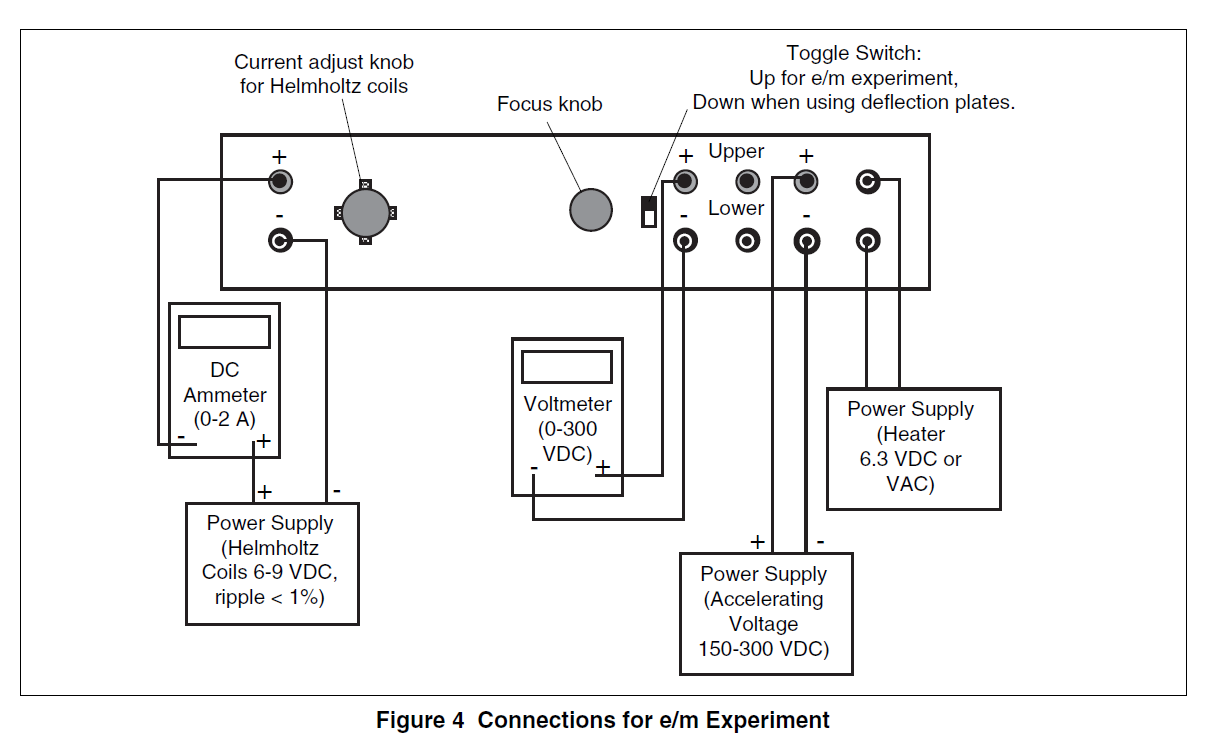
\includegraphics[width = 0.95\linewidth]{PASCO.png}% Here is how to import EPS art
	\caption{\label{fig:PASCO}실험 장비 연결 구성}
\end{figure}

이 때 측정시 전자빔의 반지름은 frontside ruler를 이용하는 경우 아래와 같이 정확한 값이 아닌 더 축소된 값을 측정하게 된다. 따라서 Backside ruler와 비교하여 비율을 구한뒤 삼각비를 이용해 정확한 전자빔의 반지름을 측정해야함에 주의한다.

\begin{figure}[htbp]
	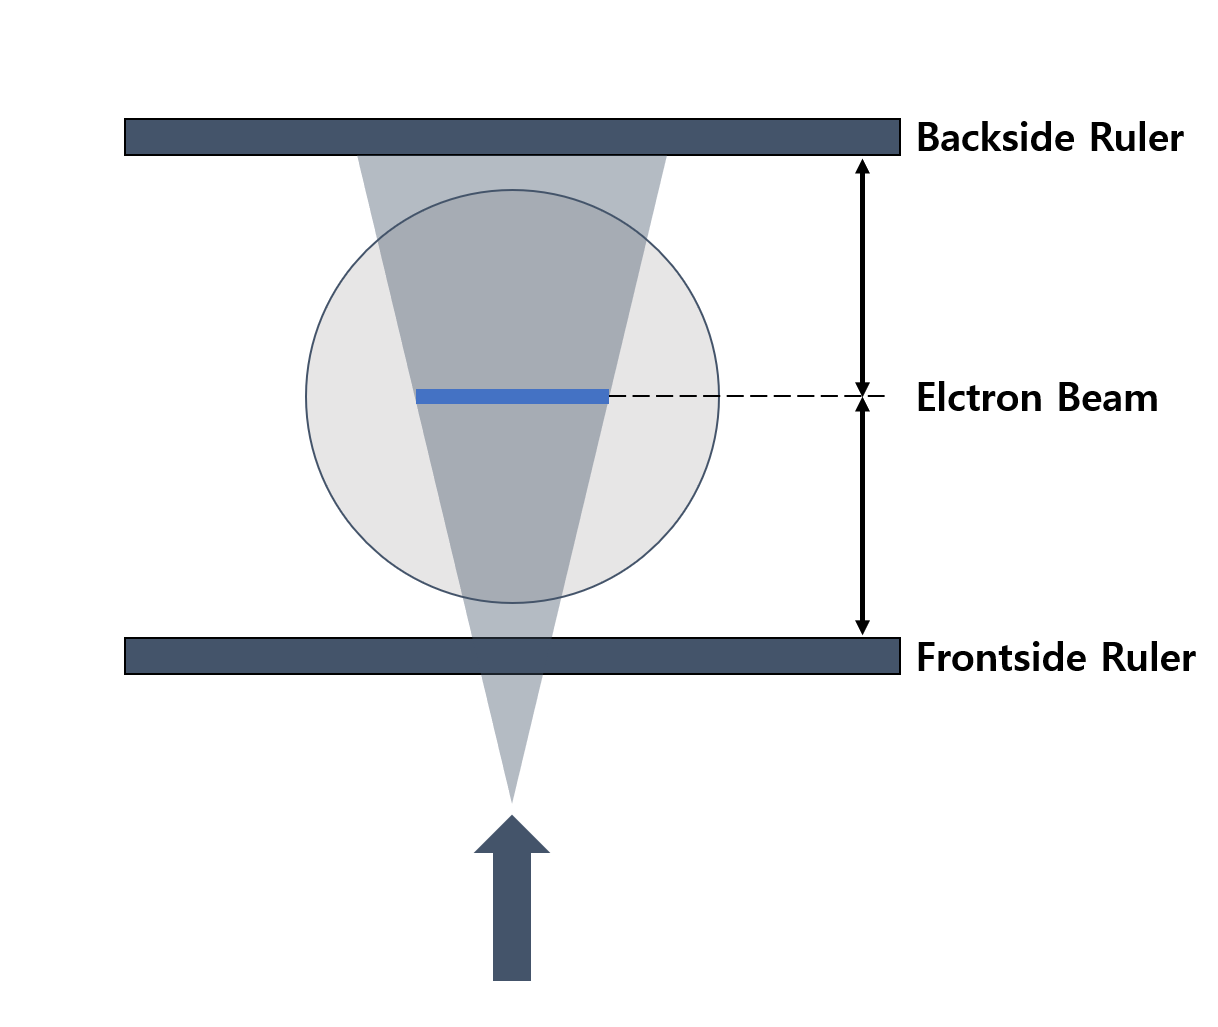
\includegraphics[width = 0.95\linewidth]{MEAS.png}% Here is how to import EPS art
	\caption{\label{fig:MEAS}전자빔 반지름 측정 모식도}
\end{figure}

\section{\label{sec:level1}Results}
각각의 전압에서 측정된 전류대비 반지름은 아래와 같다. 단, 이 때 backside ruler와 frontside ruler의 비는 $1:2$로 frontside ruler에서 측정된 값에 $1.5$를 곱하여 실제 전자빔의 반지름을 추산하였다. 또한 오차범위는 error propagation을 이용해 계산하였다.

\begin{figure}[htbp]
	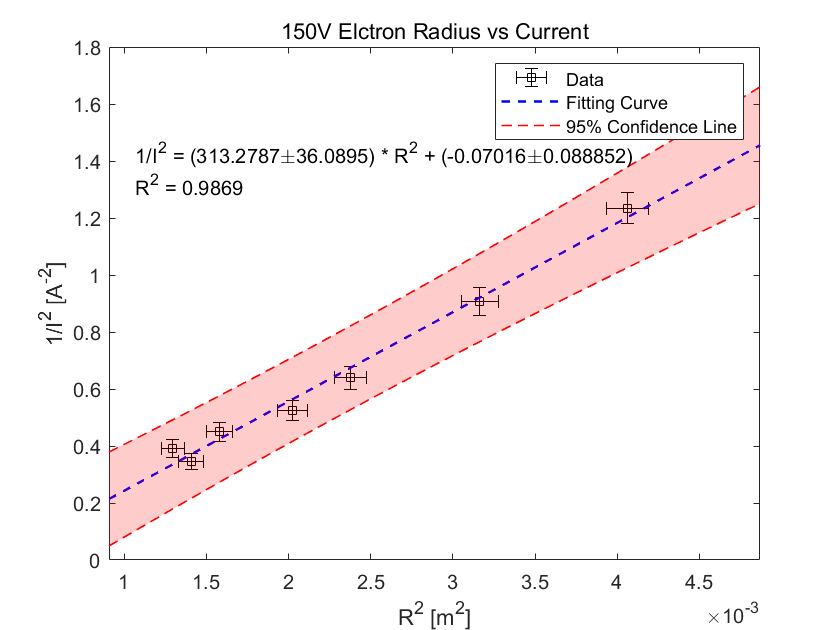
\includegraphics[width = 0.95\linewidth]{150V.png}% Here is how to import EPS art
	\caption{\label{fig:150V}$150V$로 가속하였을 때 전자빔의 반지름과 전류 관계}
\end{figure}
\begin{figure}[htbp]
	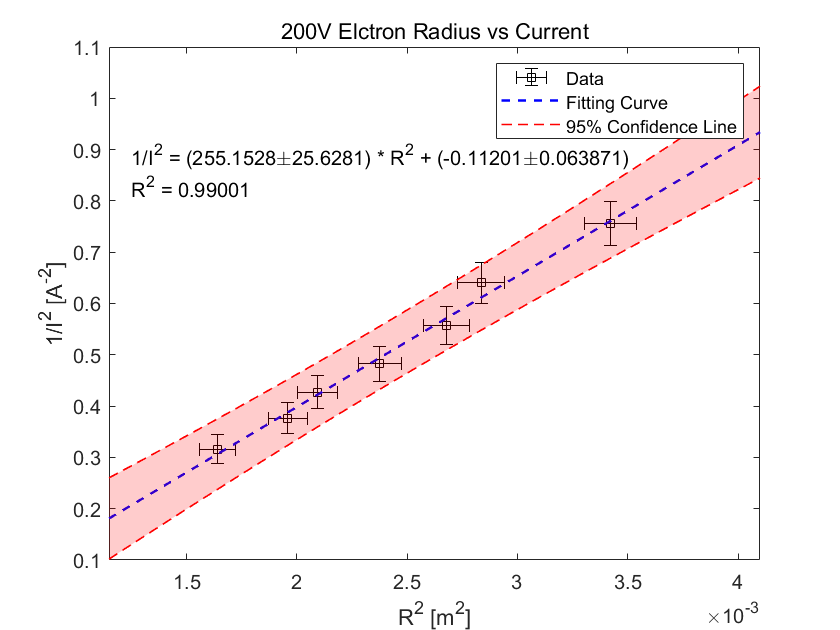
\includegraphics[width = 0.95\linewidth]{200V.png}% Here is how to import EPS art
	\caption{\label{fig:200V}$200V$로 가속하였을 때 전자빔의 반지름과 전류 관계}
\end{figure}

이 때 측정된 각각의 비전하는 Tab.\ref{tab:findat}과 같다. 이 때 오차는 기울기의 분산을 이용해 계산하였으며 $C$ 값은 $7.8\times 10^{-4}T/A$을 이용해 계산하였다.
\begin{table}[]
\begin{tabular}{c|c|c} \hline \hline
 & $150V$ & $200V$ \\ \hline
측정값[$C/kg$] & $1.54\times 10^{11}$ & $1.67\times 10^{11}$ \\ \hline
오차 [$C/kg$]& $0.18\times 10^{11}$ &  $0.17\times 10^{11}$ \\ \hline \hline
\end{tabular}
\caption{\label{tab:findat}측정된 비전하}
\end{table}

\section{\label{sec:level1}Conclusion and Discussion}
잘 알려진 전하비 값은 $1.76\times 10^{11}C/kg$으로 측정된 전하비 값은 모두 $10\%$ 내외의 오차를 가진다. 또한 선형회귀의 $R^{2}$값이 모두 $1$에 매우 가까운 값이므로 재현도 또한 매우 높다고 할 수 있다.\\ 

실험에서 나타날 수 있는 오차로는 정확하지 않은 자기장 값, 그리고 나선형태를 띠고 움직이는 전자를 고려할 수 있다. 첫번째의 경우 처음에 계산한 자기장 값은 중심에서 벗어나도 큰 오차를 주지 않는다. 또한 첫번째, 두번째 오차 요소는 전하비를 더 큰 값으로 측정되도록 하는 오차이므로 본 실험에서의 주요한 오차 요인이 아님을 알 수 있다.\\

따라서 해당 실험에서 나타난 주요한 오차 요인은 측정된 전자빔의 반지름 측정값의 불확정성 때문이다. 전자빔이 둥그런 유리구 내에 있어 직접 정확한 반지름을 측정하기에 어려움이 있어 앞, 뒤 반지름을 측정한 뒤 중간값을 취하는 방식으로 반지름을 계산하였다. 하지만 정확한 전자빔을 보는 위치에 따라 거리값은 크게 변화하므로 해당 방식이 항상 정확한 값을 나타낸다고 할 수 없다. 예를 들어 전자빔이 두 자의 중간이 아닌 $0.4$배의 위치에 있는 경우 측정값은 $14\%$ 변화하게 된다. 따라서 정확한 전자빔의 반지름을 측정하기 위해 납작한 형태의 전자빔을 이용해야만 한다.

\section{\label{sec:level1}Reference}
[1] S.M. Sze, Y. Li, and K.K. Ng, \textit{Physics of Semiconductor Devices} (Wiley-Interscience, Hoboken, , 2021). 

[2] Griffiths, \textit{Introduction to Electrodynamics} (Cambridge University Press, 2017). 

[3] D. Halliday, R. Resnick, J. Walker, and S.-B. Liao, \textit{Fundamentals of Physics} (Wiley, Hoboken, NJ, 2013). 

\end{document}
%
% ****** End of file apssamp.tex ******
